\documentclass[]{beamer}

\mode<presentation> {

%\usetheme{default}
%\usetheme{AnnArbor}
%\usetheme{Antibes}
%\usetheme{Bergen}
%\usetheme{Berkeley}
\usetheme{Berlin} %+
%\usetheme{Boadilla}
%\usetheme{CambridgeUS} %-
%\usetheme{Copenhagen}
%\usetheme{Darmstadt}
%\usetheme{Dresden}
% \usetheme{Frankfurt} %+
%\usetheme{Goettingen}
%\usetheme{Hannover}
%\usetheme{Ilmenau}
%\usetheme{JuanLesPins}
%\usetheme{Luebeck}
% \usetheme{Madrid}      
%\usetheme{Malmoe}
%\usetheme{Marburg}
%\usetheme{Montpellier}
%\usetheme{PaloAlto}
%\usetheme{Pittsburgh}
% \usetheme{Rochester} %min
% \usetheme{Singapore}
%\usetheme{Szeged}
%\usetheme{Warsaw}

% As well as themes, the Beamer class has a number of color themes
% for any slide theme. Uncomment each of these in turn to see how it
% changes the colors of your current slide theme.

%\usecolortheme{albatross}
%\usecolortheme{beaver}
%\usecolortheme{beetle}
%\usecolortheme{crane}
%\usecolortheme{dolphin}
%\usecolortheme{dove}
% \usecolortheme{fly}
%\usecolortheme{lily}
%\usecolortheme{orchid}
% \usecolortheme{rose}
% \usecolortheme{seagull}
%\usecolortheme{seahorse}
\usecolortheme{whale}
%\usecolortheme{wolverine}

%\setbeamertemplate{footline} % To remove the footer line in all slides uncomment this line
%\setbeamertemplate{footline}[frame number] % To replace the footer line in all slides with a simple slide count uncomment this line

\setbeamertemplate{navigation symbols}{} % To remove the navigation symbols from the bottom of all slides uncomment this line

\setbeamercovered{transparent} % Fait apparaître les animations en grisé (utile pour la conception, mais peut être commenté lors de la remise du document final)

% Pour utiliser une police à empattements partout
\usefonttheme{serif}

% Pour rajouter la numérotation des frames dans les pieds de page
\newcommand*\oldmacro{}%
\let\oldmacro\insertshorttitle%
\renewcommand*\insertshorttitle{%
  \oldmacro\hfill%
  \insertframenumber\,/\,\inserttotalframenumber}

}

% для нумерации картинок
\setbeamertemplate{caption}[numbered]


\setbeamertemplate{headline}
{%
  % \begin{beamercolorbox}[colsep=1.5pt]{upper separation line head}
  % \end{beamercolorbox}
  \begin{beamercolorbox}{section in head/foot}
    \vskip0pt\insertnavigation{\paperwidth}\vskip2pt
  \end{beamercolorbox}%
  % \begin{beamercolorbox}[colsep=1.5pt]{lower separation line head}
  % \end{beamercolorbox}
}

\usepackage[T2A]{fontenc}
\usepackage[utf8]{inputenc}
\usepackage[english]{babel}
\usepackage{hyperref}     % ТАК_НУЖНО
\hypersetup{unicode=true} % ТАК_НУЖНО
\usepackage{amsmath}
\usepackage{amssymb,textcomp, esvect,esint}
\usepackage{amsfonts}
\usepackage{amsthm}
\usepackage{graphicx}
\usepackage{indentfirst}
\usepackage{xcolor}
% \usepackage{enumitem} %--- ломал нумерацию!?

\usepackage{graphicx}
\usepackage{booktabs}
\usepackage{caption}
\usepackage{listings}
\usepackage{tikz}
\usepackage{xcolor}



\usepackage{media9}
\usepackage{animate}
\usepackage{threeparttable}
\usepackage{pifont}


\usepackage{import}
\usepackage{xifthen}
\usepackage{pdfpages}
\usepackage{transparent}

\usepackage[skip=1pt]{caption}
% add (renew) commands

\renewcommand{\Im}{\mathop{\mathrm{Im}}\nolimits}
\renewcommand{\Re}{\mathop{\mathrm{Re}}\nolimits}

\renewcommand{\d}{\, d}
\renewcommand{\leq}{\leqslant}
\renewcommand{\geq}{\geqslant}
\renewcommand{\l}{\left}
\renewcommand{\r}{\right}

\newcommand{\vc}[1]{\mbox{\boldmath $#1$}}
\newcommand{\T}{^{\text{T}}}


\newcommand{\diag}{\mathop{\mathrm{diag}}\nolimits}
\newcommand{\cl}{\mathop{\mathrm{cl}}\nolimits}
\newcommand{\grad}{\mathop{\mathrm{grad}}\nolimits}
\renewcommand{\div}{\mathop{\mathrm{div}}\nolimits}
\newcommand{\rot}{\mathop{\mathrm{rot}}\nolimits}
\newcommand{\Ker}{\mathop{\mathrm{Ker}}\nolimits}
\newcommand{\Spec}{\mathop{\mathrm{Spec}}\nolimits}
\newcommand{\sign}{\mathop{\mathrm{sign}}\nolimits}
\newcommand{\tr}{\mathop{\mathrm{tr}}\nolimits}
\newcommand{\rg}{\mathop{\mathrm{rg}}\nolimits}


\newcommand{\DS}{\mathcal D\left(\mathbb{R}\right)}
\newcommand{\QED}{\textnormal{Q. E. D.}}
\newcommand{\dseq}{\overset{\mathcal D'}{=}}
\newcommand{\dto}{\overset{\mathcal D'}{\to}}


\newcommand{\const}{\text{const}}
\newcommand{\xmark}{\ding{55}}


\newenvironment{uproof}{
% \begin{comment}
\par \color{ugray}
\begin{proof}[$\triangle$]
}{
\end{proof} \par
% \end{comment}
}


\newcommand{\bhat}{\overset{\text{\scalebox{0.8}[0.5]{\rotatebox[origin=c]{180}{$\wedge$}}}}}

\newcommand{\cf}[1]{\text{\raisebox{1.5pt}{$\scalebox{1.3}{$\chi$}$}}_{#1}}

\newcommand{\supp}{\mathop{\mathrm{supp}}\nolimits}
\newcommand{\si}{\mathop{\mathrm{Si}}\nolimits}

\newcommand{\rr}{\rightrightarrows}

% \newcommand{\sbsnum}[2]{
%     \setcounter{subsection}{\the\numexpr #1 - 1 \relax}
%     \subsection{#2}
% }

% Секции и сабсекции
% \definecolor{darkblue}{HTML}{000099}
% \newcommand{\sbs}[1]{\subsection{\textcolor{darkblue}{#1}}}
% \renewcommand{\sec}[1]{\section{\textcolor{darkblue}{#1}}}
\newcommand{\sbs}[2]{
\setcounter{subsection}{\numexpr #1 - 1 \relax}
    \textcolor{ugreen}{
        \subsection{#2}
        }
}


% \newcommand{\progressbar}{%
	\pgfmathsetmacro{\slidewidth}{\paperwidth}
	\pgfmathsetmacro{\progressstep}{\paperwidth/\inserttotalframenumber}
	\pgfmathsetmacro{\progresspos}{(\insertframenumber - 0.5) * \progressstep}
	\begin{tikzpicture}[scale = 0.035, line width = 1ex]
		\node[inner sep=0pt] (cat) at (\progresspos,0)	{
\includegraphics[width=30pt]{settings/cat.png}};
		\path[red] (0,0) -- (\slidewidth,0);
	\end{tikzpicture}
}

\makeatletter
\setbeamertemplate{footline}
{
\hfill \progressbar%
  \leavevmode%
  \hbox{%
  \begin{beamercolorbox}[wd=.433333\paperwidth,ht=2.25ex,dp=1ex,center]{section in head/foot}%
    \usebeamerfont{author in head/foot}\insertshortauthor~~\beamer@ifempty{\insertshortinstitute}{}{(\insertshortinstitute)}
  \end{beamercolorbox}%
  \begin{beamercolorbox}[wd=.333333\paperwidth,ht=2.25ex,dp=1ex,center]{section in head/foot}%
    \usebeamerfont{title in head/foot}\insertshorttitle
  \end{beamercolorbox}%
  \begin{beamercolorbox}[wd=.333333\paperwidth,ht=2.25ex,dp=1ex,right]{section in head/foot}%
    % \usebeamerfont{date in head/foot}\insertshortdate{}\hspace*{2em}
    % \insertframenumber{} / \inserttotalframenumber\hspace*{2ex} 
  \end{beamercolorbox}}%
  \vskip0pt%
}

\setbeamertemplate{caption}[numbered]
\title[Choice Question]{Implementations of dynamic chaos \\
in different optical systems}

\author{
Khoruzhii K., Primak E.}
\institute[MIPT]

\begin{document}
\date{1.06.2021}
\maketitle




\section{Chaos}

\frame{
\textit{Globally} we would like to 
transmit a high-frequency signal in encrypted form.

\phantom{42}

Here we will consider the following steps towards the goal:
\begin{itemize}
    \iitem{dynamical chaos and synchronization \\ 
    (to encrypt and decrypt signal);}
    \iitem{theory of the laser evolution and its adaptation under our needs;}
    \iitem{modeling theoretical equations and investigating chaos parameters;}
    \iitem{realization of the positive feedback in laser: \\
     theory, modeling and the experiment.}
\end{itemize}
 \frametitle{Goals}}

\frame{

  Map\footnote{
    W. Hirsch, S. Smale, Introduction to Chaos.
} $f$ is \textbf{chaotic}, if \\
\begin{itemize}
    \iitem{periodic orbits are dense everywhere;}
    \iitem{orbits are mixed;}
    \iitem{$f$ sensitive to the initial conditions.}
\end{itemize}

\vspace{-5mm}
\begin{figure}[h]
    \centering
    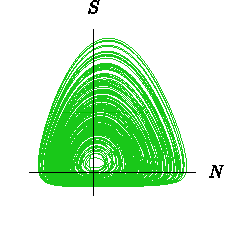
\includegraphics[width=0.25\textwidth]{figures/attractor.pdf}
    \hspace{5 mm}
    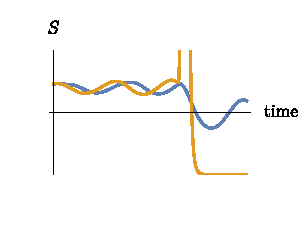
\includegraphics[width=0.35\textwidth]{figures/ics.pdf}
    %\caption{}
    %\label{fig:}
\end{figure}

\vspace{-5mm}
\begin{minipage}{0.35\textwidth}
      Possible applications:
\end{minipage}
\hfill
\begin{minipage}{0.63\textwidth}
    \begin{itemize}
        \iitem{random numbers generation;}
        \iitem{signal encryption.}
    \end{itemize}
\end{minipage}


 \frametitle{Definition of dynamic chaos and applications}}

\frame{



Possible\footnote{
    M. Pecora, L. Carroll, Synchronization in Chaotic Systems, 1990.
}  synchronization of chaotic systems:

% \hspace{-5mm}
\begin{minipage}{0.65\textwidth}
        \textit{enough} to transmit\\
        \phantom{python} part of the signal;\\
        \phantom{python} configure system parameters. 
\end{minipage}
\hfill
\begin{minipage}{0.3\textwidth}
    \begin{center}
        \incfig{scheme}
    \end{center}
\end{minipage}


\phantom{42}

The use of optics to transmit the signal allows to achieve a greater bandwidth of the channel. 

\phantom{42}

UHFO (ultrahight frequency oscillations) is a characteristic to optic systems.

 \frametitle{Synchronization}}

% 

\frame{
The beam goes to the film through the optical fiber:

\phantom{42}

\begin{minipage}{0.45\textwidth}
    \begin{center}
        \incfig{scheme8}    
    \end{center}
\end{minipage}
\hfill
\begin{minipage}{0.45\textwidth}
    \begin{figure}[h]
        \centering
        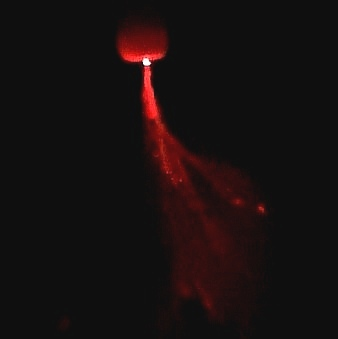
\includegraphics[width=0.99\textwidth]{figures/photo3.jpg}
        %\caption{}
        %\label{fig:}
    \end{figure}
\end{minipage}

\phantom{42}

Light scattering occurs most likely on micro bubbles and other inhomogeneities inside the solution. \frametitle{Experimental setup}}

\frame{


After outlet of the optical fiber ($d_{\text{core}} \sim 50 \, \mu$m) light really starts branching.

\begin{figure}[h]
    \animategraphics[loop, controls=play,width=0.52\textwidth]{20}{gifs/g2/}{1}{100} 
    \hspace{5 mm} 
    \animategraphics[loop, controls=play,width=0.3\textwidth]{20}{gifs/g1/}{1}{54} 
\end{figure}

The effect of the thickness of the film on the system dynamics is noticeable. After the time expires, the film becomes thinner, the rays are actively branched. \frametitle{Film dynamics}}

\frame{
To demonstrate branching, consider the movement of light in the environment with 
$n(x, y) = \textstyle\frac{1}{3}\left(\cos x +\cos y \right) + 2$.

% \phantom{42}

\begin{minipage}{0.6\textwidth}
      \begin{figure}[h]
      \animategraphics[loop,controls=play,width=0.99\textwidth]{20}{gifs/g3/}{1}{63}
    \end{figure}
\end{minipage}
\hfill
\begin{minipage}{0.35\textwidth}
    \begin{figure}[h]
        \centering
        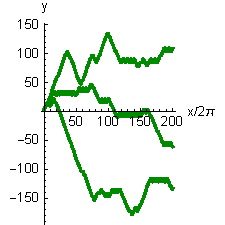
\includegraphics[width=1.0\textwidth]{figures/rnd_walk.pdf}
        %\caption{}
        %\label{fig:}
    \end{figure}

     \phantom{42}
\end{minipage}

This happens random walk across heterogeneous media. \frametitle{Modeling}}

\frame{
Walk in periodic media can be reduced to the billiard table.

\begin{minipage}{0.5\textwidth}
      \begin{figure}[h]
      \animategraphics[loop,controls=play,width=0.99\textwidth]{20}{gifs/g4/}{1}{200} 
    \end{figure}
\end{minipage}
\hfill
\begin{minipage}{0.45\textwidth}
For almost all trajectories:
    \begin{itemize}
        \item[\textcolor{mygreen}{\checkmark}] ergodic behaviour;
        \item[\textcolor{mygreen}{\checkmark}] positive Lyapunov exponent;
        % \item[\textcolor{mygreen}{\checkmark}] .
    \end{itemize}
    so we have pretty example of dynamical chaotic system.
\end{minipage}


That can be considered as a smoothed version of Lorentz gas or Sinai billiard. \frametitle{Sinai billiard}}

% \section{Laser}

\frame{
To start the laser idea we need to obtain:
\begin{itemize}
	\iitem{Solution of the Schr\"odinger equation in a semiconductor medium for the wavefunction of an electron;}
	\iitem{Induced polarization for distribution of holes and electrons in a semiconductor;}
	\iitem{Interaction of electrons in a semiconductor with an wave equation and outer electric field.}
\end{itemize}
 \frametitle{The concept of a semiconductor laser}}

\frame{
We will need the Schr\"odinger equation:
\begin{equation*}
	H_{\text{crystal}} \Psi_n(\vc{r}) = \left[\frac{\vc{p}^2}{2 m_0} + U_p(\vc{r})\right] \Psi_n(\vc{r})
\end{equation*}
where $\vc{p} = - i \hbar \nabla$ is the momentum operator, $m_0$ is the free electron mass, $U_p(\vc{r})$ is th periodic potential of the bulk semiconductor.

The solution is the Bloch function:
\begin{equation*}
	\Psi_{n, \smallvc{k}}(\vc{r}) = u_{n, \smallvc{k}}(\vc{r}) \frac{1}{\sqrt{V}} e^{i \smallvc{k} \cdot \smallvc{r}}.
\end{equation*}
 \frametitle{Electronic states in a semiconductor}}

\frame{
In case of an optical field the Hamiltonian changes to
\begin{equation*}
	H = \frac{[\vc{p} + e \vc{A}(\vc{r}, t)]^2}{2 m_0} + U_p(\vc{r}) = H_\text{crystal} + H'
\end{equation*}
$\vc{A}(\vc{r},t)$ is the vector potential of the optical field. So the interaction Hamiltonian 
\begin{equation*}
	H' \approx \frac{e}{m_0} \vc{A}(\vc{r},t) \cdot \vc{p}.
\end{equation*} \frametitle{Hamilton in an outer field}}

\frame{
For y-propagating field: $E(\vc{r}, t) = \frac{1}{2} E_0 e^{i (\beta y - \omega t)} + \const$ the Hamiltonian is
\begin{equation*}
	H' = \frac{1}{2} \mu(k_q,x,z) [E_0 e^{i (\beta y - \omega t)} + \const]
\end{equation*}
where $\mu$ is the transition matrix that describes the semiconductor, $k_q$ -- quantized wavevector of the electron. \frametitle{Hamilton in an outer field}}

\frame{
As one can obtain after rewritten density matrix in terms of carrier distributions, and in order avoid irrelevantly enormous formulas we get polarization as:
\begin{equation*}
	\mathcal{P}_{in}(\vc{r}, t) = \frac{1}{2} \mathcal{P}_{in,0} e^{i (\beta y - \omega t)} + \const =
\end{equation*}
\begin{equation*}
	= - \sum \frac{\xi(\vc{r},k_q, x, z)}{V(k_q, x, z)}[\rho_{eh}(k_q, x, z)\mu(k_q, x, z) + \const]	
\end{equation*}
where $V(k_q, x, z)$ is the confinement volume of electrons and holes and
\begin{equation*}
	\xi(\vc{r}, k_q, x, z) = 
	\left\{ \begin{aligned}
		&1, \ \vc{r} \text{ inside V}\\
		&0, \ \vc{r} \text{ outside V}
	\end{aligned}
	\right.
\end{equation*}

 \frametitle{Induced polarization in an outer field}}

\frame{
For the wave porpagating along the y direction in active layer the equation is:
\begin{equation}
	\triangle E(\vc{r},t) - \mu_0 \varepsilon(\vc{r}) \frac{\partial^2}{\partial t^2} E(\vc{r}, t) = \mu_0 \frac{\partial^2}{\partial t^2} P_{in}(\vc{r},t)
	\label{1.46}
\end{equation}
The partial solution for this equation we will be searching in a form of
\begin{equation*}
	E(\vc{r}, t) = A_0(t) E_{\text{eig}}(x,z) = \frac{1}{2} E_0 e^{i (\beta y - \omega t)} + \const.
\end{equation*} \frametitle{Injection the light}}

\frame{
Substituting in wave equation\eqref{1.46} the obtained polarization and solution for $E(\vc{r}, t)$ and assuming that $A(t)$ changes slowly we get
\begin{equation}
	\frac{d A_0}{d t} = \frac{i \omega}{2 \varepsilon_0 n_r^2} A_0 \sum_{k_q, x, z}\Gamma_{MD} \frac{1}{V_{MD}} |\mu(k_q, x, z)|^2[\rho_{ee} + \rho_{hh} - 1]
\end{equation}
where 
\begin{equation*}
	\Gamma_{MD} = \frac{\varepsilon(x,z) |E_0(x,z)|^2}{\iint \varepsilon(x,z) |E_0(x,z)|^2 dx d z}\bigg|_{x,z=0,0}
\end{equation*}
is a \textit{dimensional coupling factor}. \frametitle{Partial solution part}}

\frame{
Now we can rewrite
\begin{equation}
	\frac{d A_0}{d t} = \frac{1}{2} v_g [\Gamma_{MD}G - i \Gamma_{MD} N_r]A_0,
\end{equation}
where $v_g = c/n_r$ for $c$ -- the speed of light in vacuum, and $n_{r}$ -- refraction coefficient. We will call the \textit{gain coefficient} $g = \Gamma_{MD}G$.
From Schr\"odinger equation we obtain the photon density as:
\begin{equation*}
	S = \frac{1}{2} \frac{\varepsilon_0 n_r^2 |A_0 E(0)|^2}{E_0}.
\end{equation*} \frametitle{Getting the solution}}

\frame{
Using the equation for $A_0$ we obtain for the photon density (real part):
\begin{equation}
	\frac{d S}{d t} = v_g \Gamma_{MD} G(E) S.
\end{equation}

Total optical power in the active region:
\begin{equation*}
	-\int E(\vc{r},t) \frac{d \mathcal{P}_{in}(\vc{r},t)}{d t} d \vc{r} = - \hbar \omega V_{MD} \frac{d N_{MD}}{d t},
\end{equation*}
which leads to electrons (holes) density (complex part):
\begin{equation}
	\frac{d N_{MD}}{d t} = - v_g G(E) S.
\end{equation} \frametitle{The laser equations}}

\frame{
Irrelevantly enormous
formulas if someone really need it:

\begin{equation*}
	\frac{d}{d t}[\rho_{ee}(k_q, x, z)] = \frac{i}{\hbar}[H' \rho_{eh}(k_q, x, z) - \const] - \frac{\rho_{ee}(k_q, x, z) - f_e}{\tau_e},
\end{equation*}
\begin{equation*}
	\frac{d}{d t}[\rho_{hh}(k_q, x, z)] = \frac{i}{\hbar}[H' \rho_{eh}(k_q, x, z) - \const] - \frac{\rho_{hh}(k_q, x, z) - f_e}{\tau_e},
\end{equation*}
\begin{equation*}
	\frac{d}{d t}[\rho_{eh}(k_q, x, z)] = \frac{i}{\hbar} H'[\rho_{ee} + \rho_{hh} - 1] - \frac{i}{\hbar} E_{tr} \rho_{e h} - \frac{\rho_{eh}}{T_{deph}}.
\end{equation*} \frametitle{Carrier density in an outer field}}

\frame{
And from the previous equation we can describe the quantum well laser behavior
\begin{equation*}
	\frac{d S}{d t} = \Gamma(0) G_0 v_g S - \frac{S}{\tau_p}. 
\end{equation*}
\begin{equation*}
	\frac{d N}{d t} = \frac{J}{e} - \frac{N}{\tau_n} - \Gamma G_0 v_g S.
\end{equation*} \frametitle{The laser equations}}


\frame{
\begin{figure}[h]
    \centering
    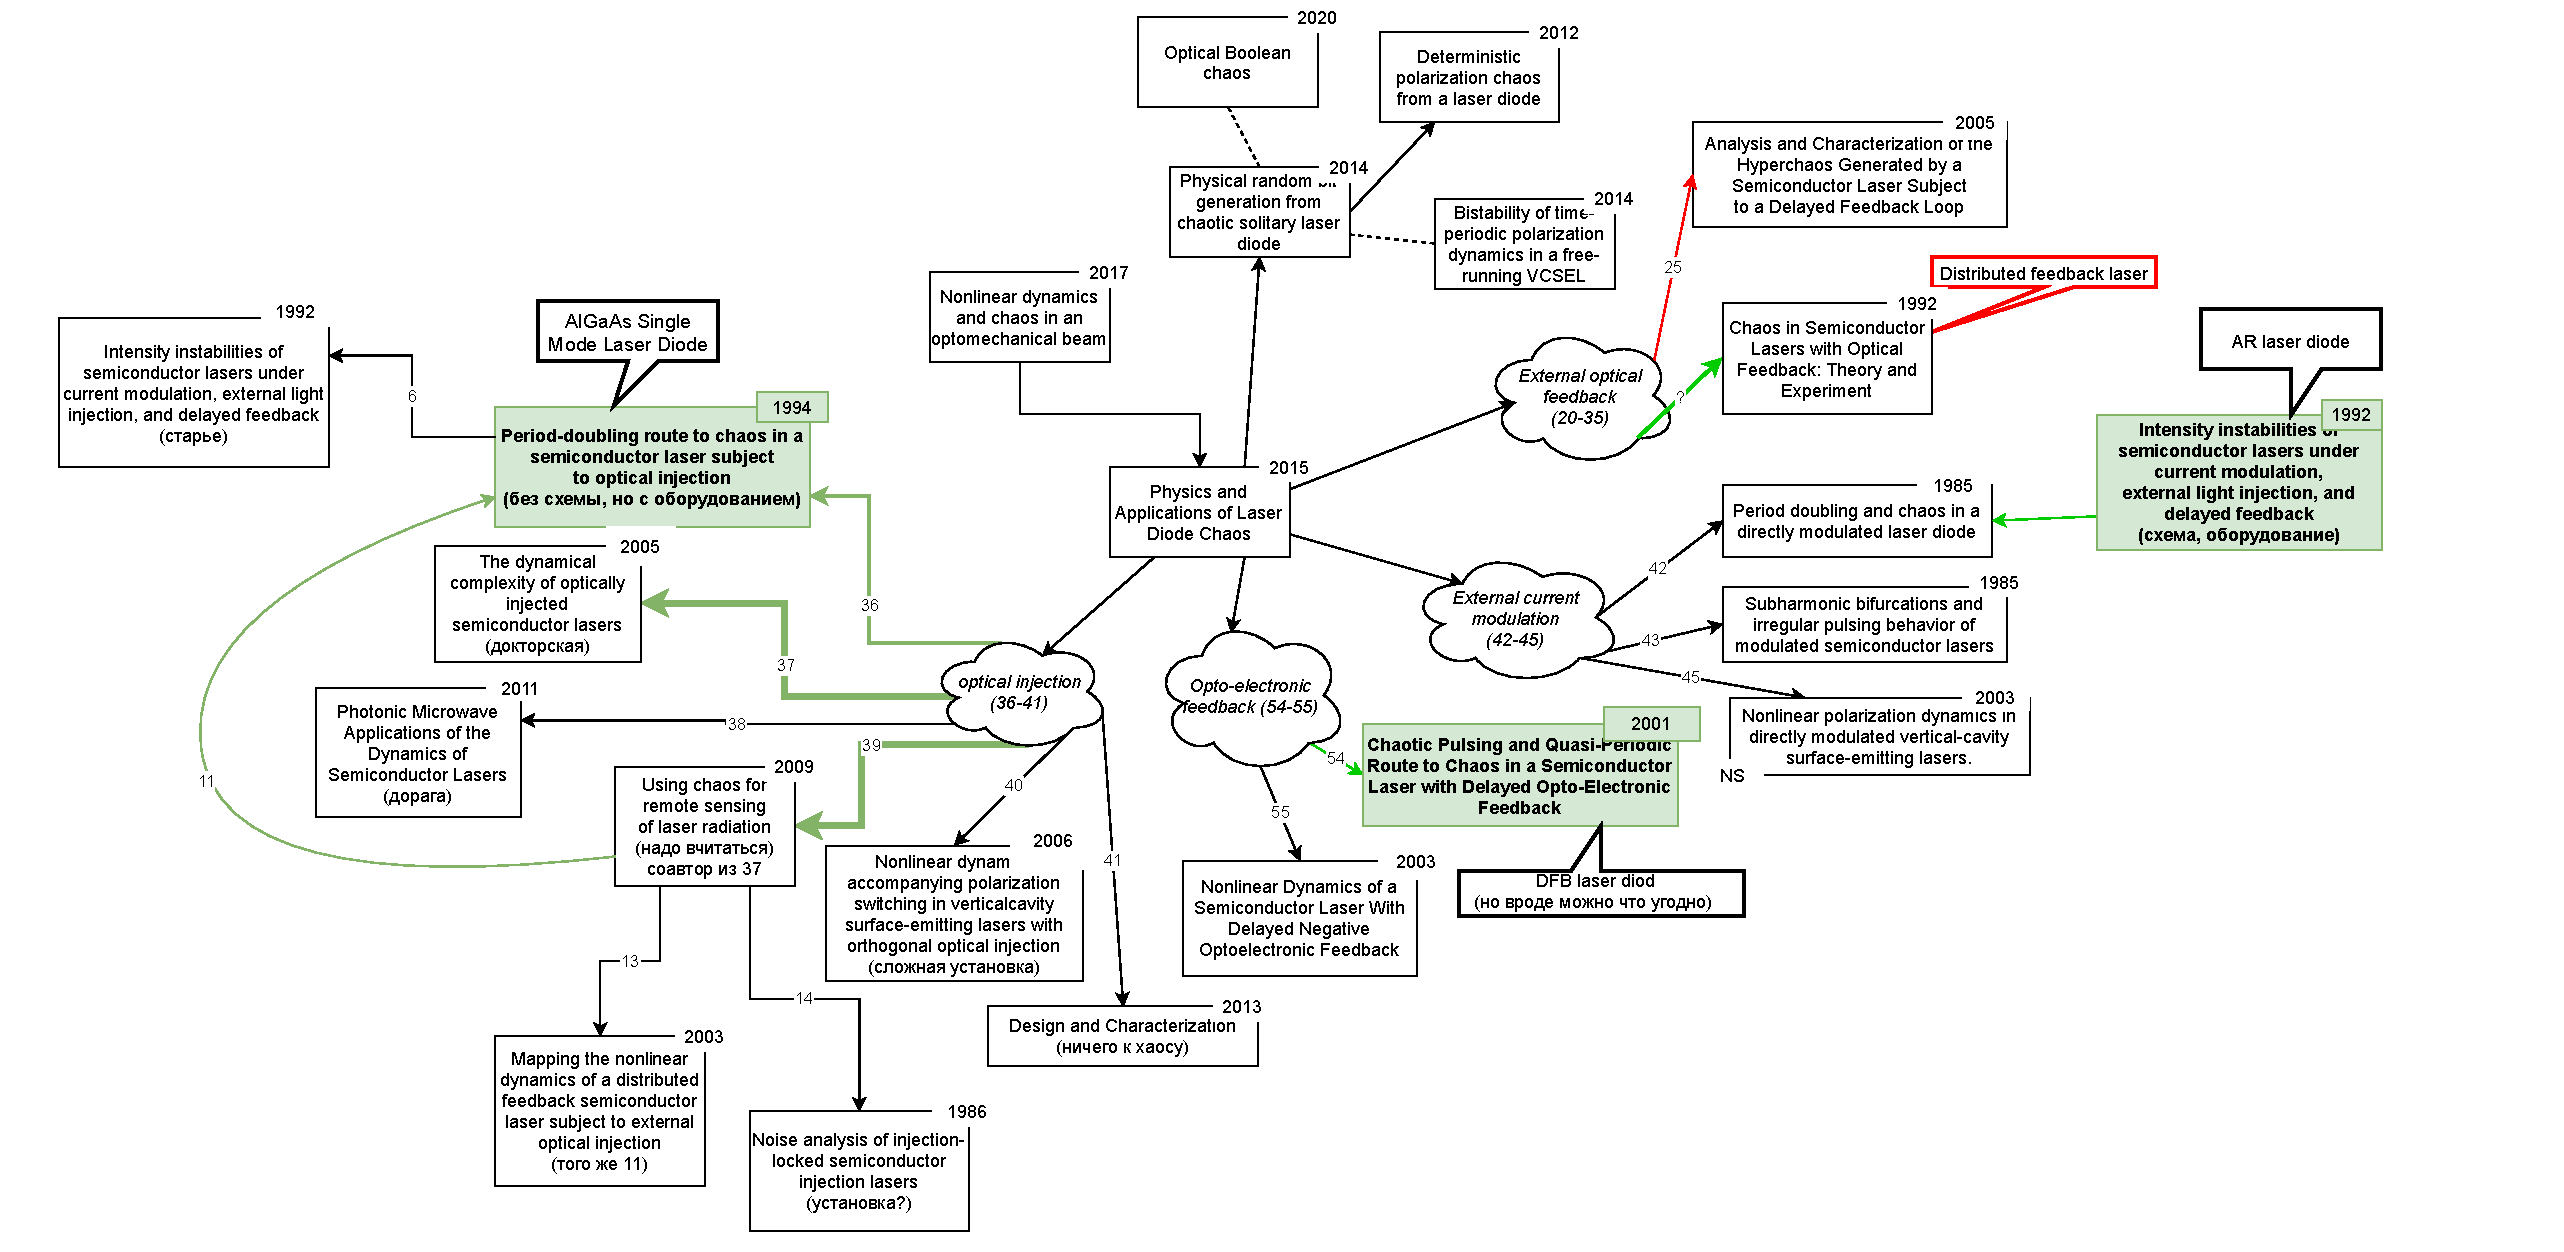
\includegraphics[width=1.1\textwidth]{images/lit_obzor_scary.pdf}
    %\caption{}
    %\label{fig:}
\end{figure}
\footnotetext{Physics and Applications of Laser Diode Chaos by
M. Sciamanna et al.
}
 \frametitle{From the root article a tree has grown}}

\frame{
\begin{minipage}{0.55\textwidth}
    \begin{figure}[h]
    \centering
    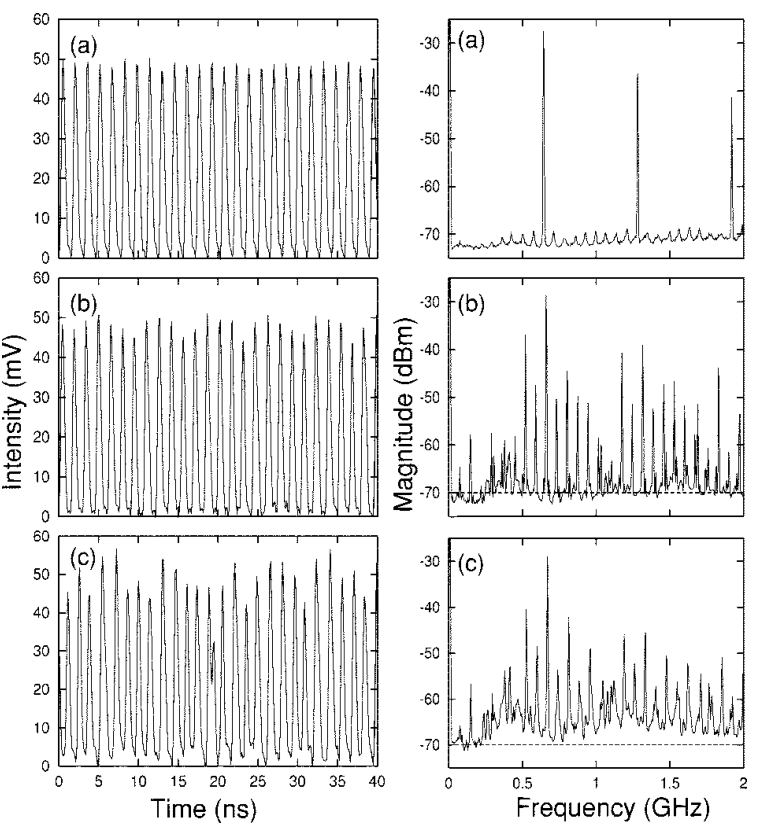
\includegraphics[width=0.9\textwidth]{images/tang_exp.png}
    % \caption{}
    %\label{fig:}
\end{figure}
\end{minipage}
\hfill
\begin{minipage}{0.35\textwidth}
	\begin{figure}
		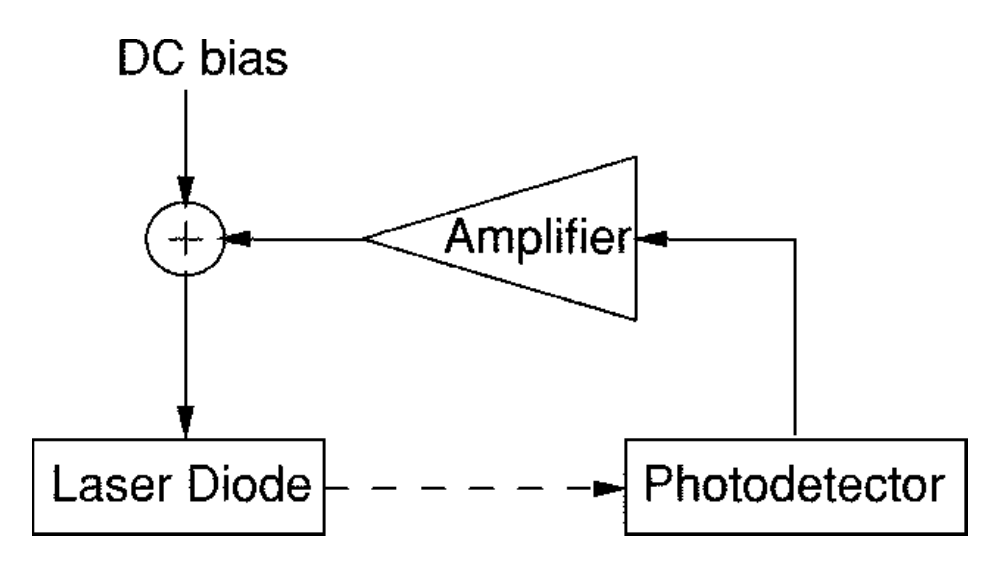
\includegraphics[width=1\textwidth]{images/tang_circr.png}
    \caption{Experimental results of the time series and power spectra of different pulsing states at different delay times.
    On a circuit dashed line represents optical path.}
	\end{figure}
\end{minipage}
\footnotetext{Chaotic Pulsing and Quasi-Periodic Route to
Chaos in a Semiconductor Laser with Delayed
Opto-Electronic Feedback
S. Tang and J. M. Liu (2001)} \frametitle{The decided variant}}

% \section{Theory}

\frame{
\begin{minipage}{0.45\textwidth}
    \begin{figure}[h]
    \centering
    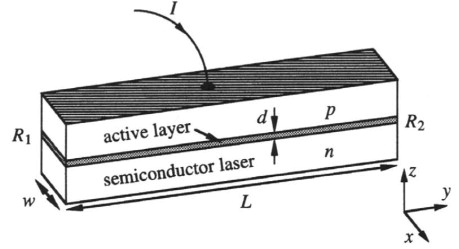
\includegraphics[width=1\textwidth]{images/semi_medium.png}
    \caption{}
    %\label{fig:}
\end{figure}
\end{minipage}
\hfill
\begin{minipage}{0.49\textwidth}
    In the active layer we obtain the Schr\"odinger equation:
    \begin{equation*}
	H_{\text{crystal}} \Psi_n(\vc{r}) = \left[\frac{\vc{p}^2}{2 m_0} + U_p(\vc{r})\right] \Psi_n(\vc{r})
\end{equation*}
\end{minipage}
 \frametitle{The
laser device geometry}}
\frame{
\textbf{Thr.} If there is no stationary points on the enclosed 2D region $G$ and some trajectory exists $\gamma \subset G$, then $\gamma$ is a closed loop path or tends to the closed one.

But there is still a hope for a chaos!

We add positive optoelectronic feedback in order to raise to 3D our equation.
\begin{align*}
	&\frac{d S}{d t} = v_g g S - \gamma_p S,\\
	&\frac{d N}{d t} = \frac{J}{e}[1 + \frac{\xi S(t-\tau)}{S_0}] - \gamma_n N - g S.
\end{align*} \frametitle{Poincar\'e-Bendixson theorem}} Женя хочет в своем рассказе вопроса по выбору это раскоментить
% \section{Theory}

\frame{
\begin{minipage}{0.45\textwidth}
    \begin{figure}[h]
    \centering
    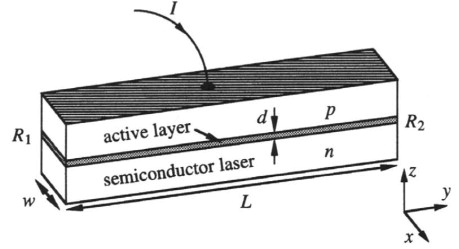
\includegraphics[width=1\textwidth]{images/semi_medium.png}
    \caption{}
    %\label{fig:}
\end{figure}
\end{minipage}
\hfill
\begin{minipage}{0.49\textwidth}
    In the active layer we obtain the Schr\"odinger equation:
    \begin{equation*}
	H_{\text{crystal}} \Psi_n(\vc{r}) = \left[\frac{\vc{p}^2}{2 m_0} + U_p(\vc{r})\right] \Psi_n(\vc{r})
\end{equation*}
\end{minipage}
 \frametitle{The
laser device geometry}}
\frame{
\textbf{Thr.} If there is no stationary points on the enclosed 2D region $G$ and some trajectory exists $\gamma \subset G$, then $\gamma$ is a closed loop path or tends to the closed one.

But there is still a hope for a chaos!

We add positive optoelectronic feedback in order to raise to 3D our equation.
\begin{align*}
	&\frac{d S}{d t} = v_g g S - \gamma_p S,\\
	&\frac{d N}{d t} = \frac{J}{e}[1 + \frac{\xi S(t-\tau)}{S_0}] - \gamma_n N - g S.
\end{align*} \frametitle{Poincar\'e-Bendixson theorem}} можно и раскоментить, но зачем теория, если она и так валяется в конце?

\section{Feedback impl.}

% \frame{
% \begin{minipage}{0.45\textwidth}
    
\end{minipage}
\hfill
\begin{minipage}{0.45\textwidth}
    \begin{center}
        \incfig{scheme2}
    \end{center}
\end{minipage}

 \frametitle{Concept}}

\frame{

After several experiments came to this scheme with the summing amplifier:
\begin{center}
    \incfig{scheme3}
\end{center}

Photodiode power is enough to not use an additional amplifier. \frametitle{Scheme}}

\frame{
For testing, the assembly was carried out on the dumping board.
\begin{center}
    \incfig{scheme4}
\end{center}

\hspace{-3mm}
\textbf{Thus, a scheme with positive feedback was implemented.} \\

\hspace{-3mm}
However, no desired oscillations were observed. \frametitle{Realization}}

\frame{

Makes sense to be in the most sensitive range, it was measured: \\
 -\ $I$-$V$ curve  for a laser \\
 -\ the dependence of the ph. diode voltage on the laser power.

\begin{figure}[h]
    % \centering
    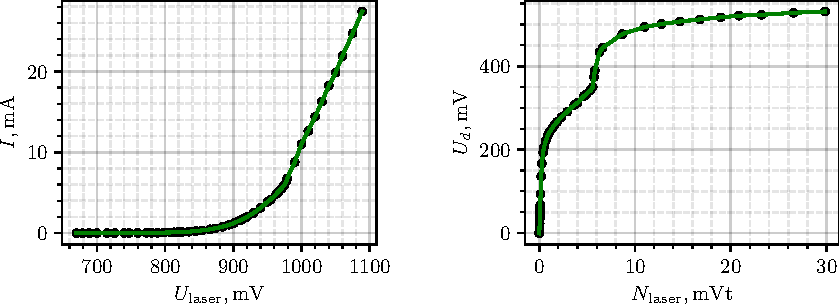
\includegraphics[width=1.0\textwidth]{figures/IV.pdf}
    %\caption{}
    %\label{fig:}
\end{figure}

So, laser voltage range of  $0.85$V selected. \frametitle{I–V curve}}

\frame{
With used amplifiers, the following oscillations at the amplifier output with DC power can be observed:

\begin{center}
    \incfig{scheme5}
\end{center}

This is due to the instability of the amplifier. 
% This instability can be eliminated by the adjustment of the scheme. 

\phantom{42}

The main problem is that desired oscillations $\sim 10$ ns. \\

\phantom{42}

We proceeded to experiments with faster amplifiers, but it is usefull to understand results of such delays.

oscillations megahertz
 \frametitle{Problems}}

% \frame{
% However, it was not possible to move to the chaotic regime in the laser. Possible cause of the problem may be
\begin{itemize}
    \iitem{parasitic capacity and inductance,}
\end{itemize}
In terms of solutions -- neatly soldered scheme.


% \phantom{42}

% A suitable amplifier, with similar properties used in the article, must come in June. \frametitle{Problems}}




\section{Modeling}

\begin{frame}
  \frametitle{Laser parameters.}
  % Unimodular, multimodular and chaotic regimes of laser work:
  \begin{columns}
    \begin{column}{.4\linewidth}
      Unmodulated laser ($\xi = 0$):
    \begin{figure}
        \centering
        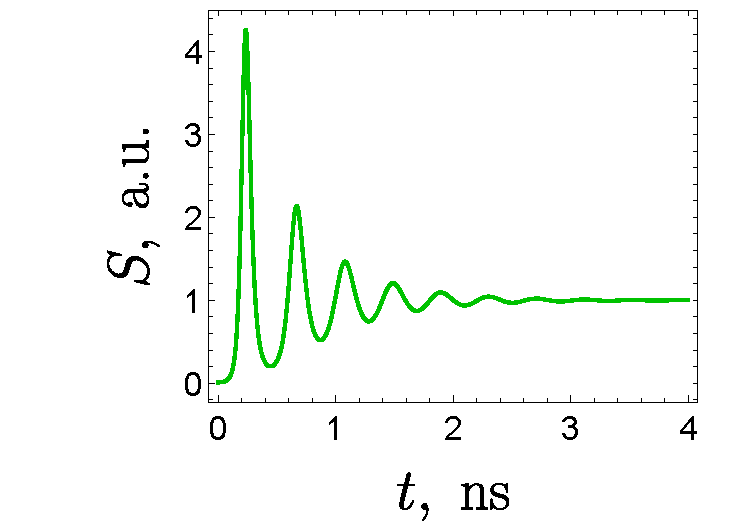
\includegraphics[width=\linewidth]{figures/laser_classic.pdf}
    \end{figure}
    
    \end{column}
    \begin{column}{.6\linewidth}
      Laser equations:
      \begin{align*}
        \frac{d S}{d t}&=-\gamma_{c} S+\Gamma g S \\
        \frac{d N}{d t}&=\frac{J}{e d}\left[1+\frac{\xi S(t-\tau)}{S_{0}}\right]-\gamma_{s} N-g S
      \end{align*}
    \end{column}
  \end{columns}

  Systems parameters:
  \begin{itemize}
    \iitem{ $f_r$ - laser relaxation frequency. For our laser: $f_r = 1.4 \div 3.2 \ \text{GHz}$.}
    \iitem{ $\tau$ - delay time. $\tau \sim f_r^{-1}$.}
    \iitem{ $\xi = 0.1$ feedback parameter.}
  \end{itemize}
  
  % Here dimensionless variable $s = \dfrac{S}{S_0}$.  
\end{frame}

\begin{frame}
  \frametitle{Chaos parameters.}
  
  % Unimodular, multimodular and chaotic regimes of laser work:
  \begin{columns}
    \begin{column}{.4\linewidth}
      \begin{figure}
        \centering
        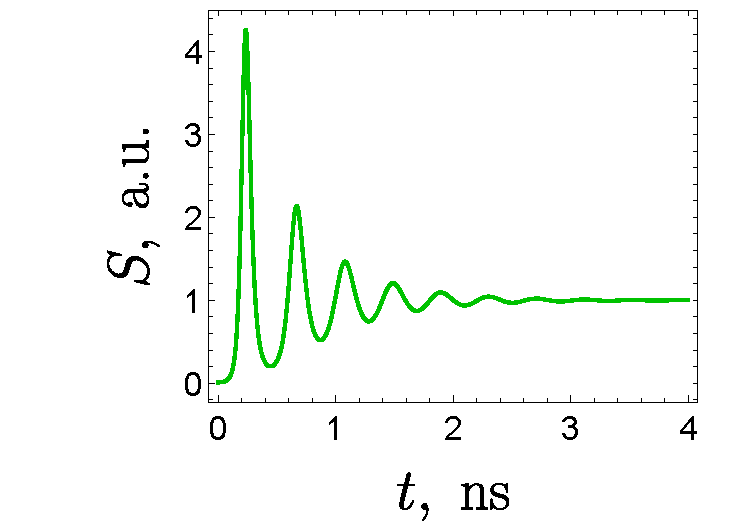
\includegraphics[width=\linewidth]{figures/laser_classic.pdf}
%        \caption{unbiased laser}
      \end{figure}
      \begin{figure}
        \centering
        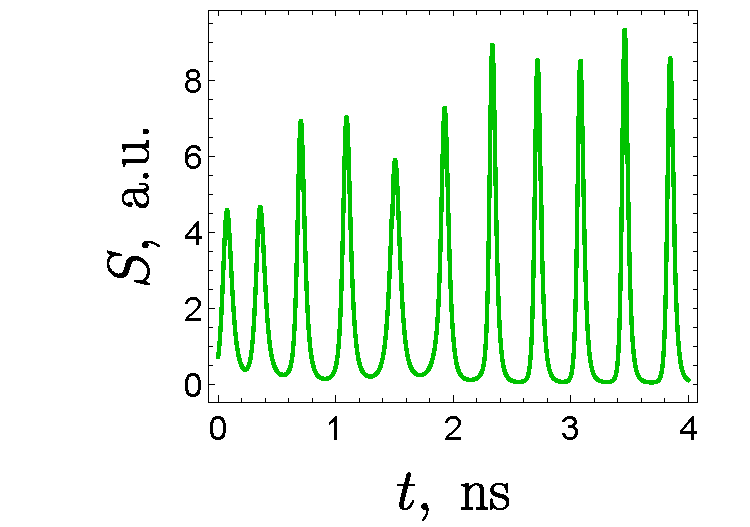
\includegraphics[width=\linewidth]{figures/laser_chaos.pdf}
      \end{figure}
      % another figure may be added with chaotic laser
    \end{column}
    \begin{column}{.6\linewidth}
      Chaos features:
      \begin{itemize}
        \iitem{ Unperiodic behaviour }
        \iitem{ Frequency doubling scenario $f \ \to \ 2 f \to \ 4f \to \dots \to \infty f$}
      \end{itemize}
      
      Chaos characteristics:
      \begin{itemize}
        \iitem{$\lambda $ -- (Lyapunov's exponent). Exponential divergence on time for close i.c.: $\Delta S (t) \approx  \Delta S (0) e^{\lambda t} $, where  $\Delta S (0) \ll S_0$.}
        \iitem{Embedded dimensions}
        \iitem{Shannon entropy}
      \end{itemize}
    \end{column}
  \end{columns}
  
  % Here dimensionless variable $s = \dfrac{S}{S_0}$.  
\end{frame}

\begin{frame}
  \frametitle{Chaos modelling. Different regimes.}
  
  % Unimodular, multimodular and chaotic regimes of laser work:
  \begin{figure}
    \centering
    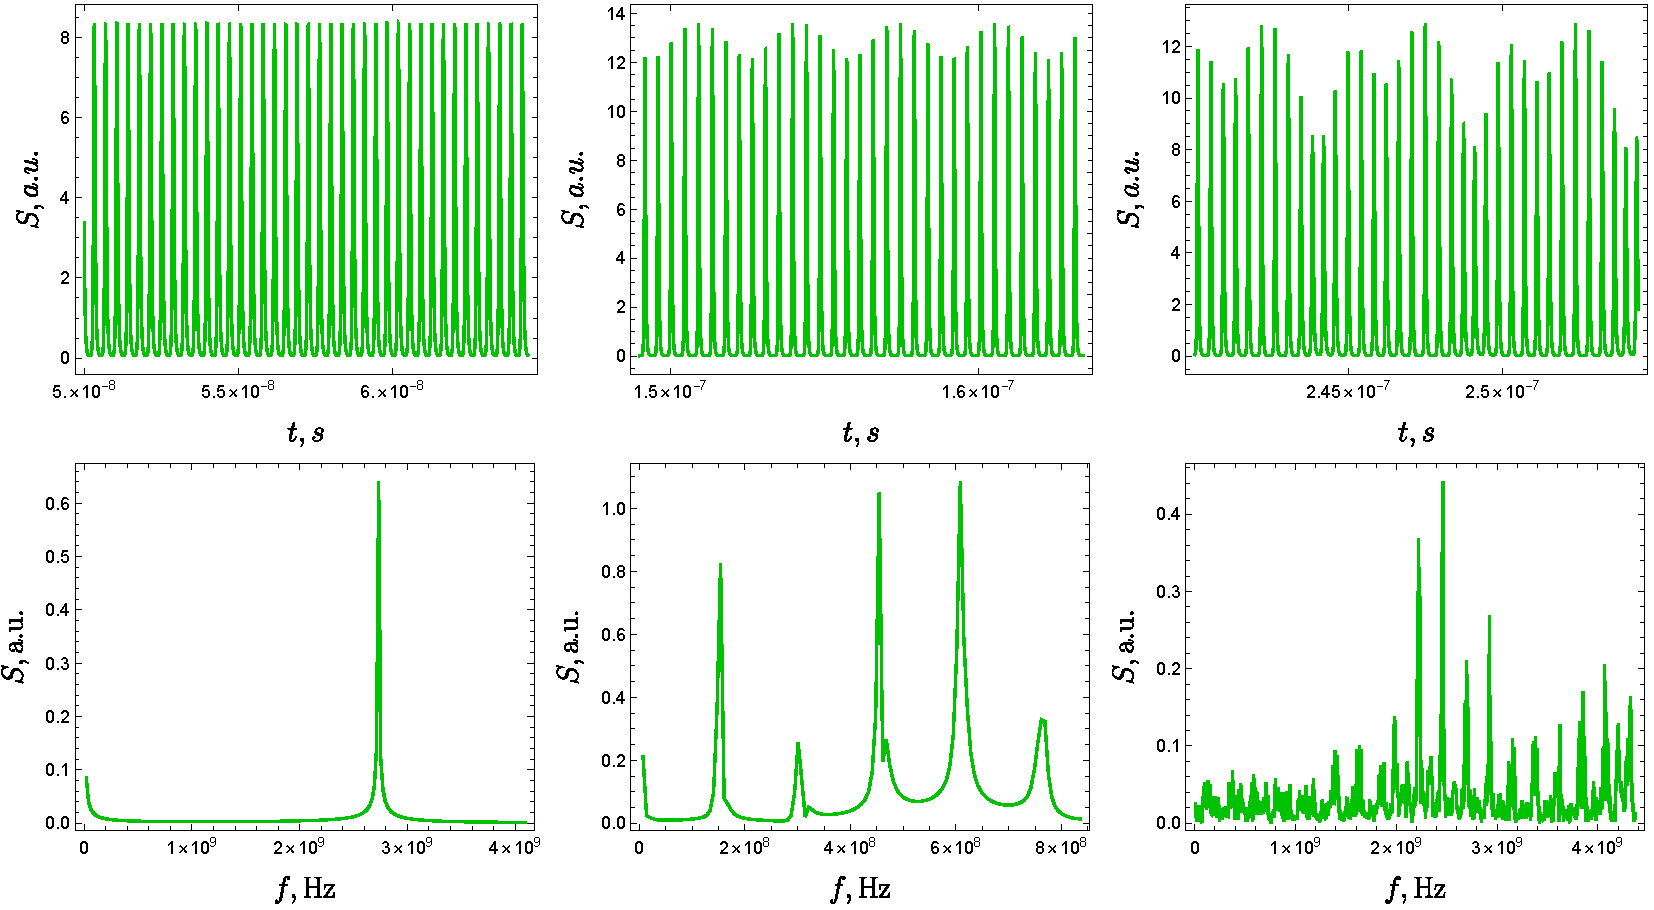
\includegraphics[width=\linewidth]{figures/chaos_and_spectra.pdf}
  \end{figure}
  
  \begin{center}
    \begin{tabular}{c|c|c}
      Delay time $\tau$:\ \ $2 \ T_r$ & $7.5 \ T_r$ & $12 \ T_r$
    \end{tabular}
  \end{center}
  
  % Here dimensionless variable $s = \dfrac{S}{S_0}$.
  
  
\end{frame}

\begin{frame}
  \frametitle{Chaos modelling.}
  Lyapunov exponents calculation for different points:
  
  $$\Delta S \sim \exp(\lambda t) \ \Rightarrow \ \log \Delta S = \lambda t + \const$$\\[5pt]
  
  \begin{figure}[h]
    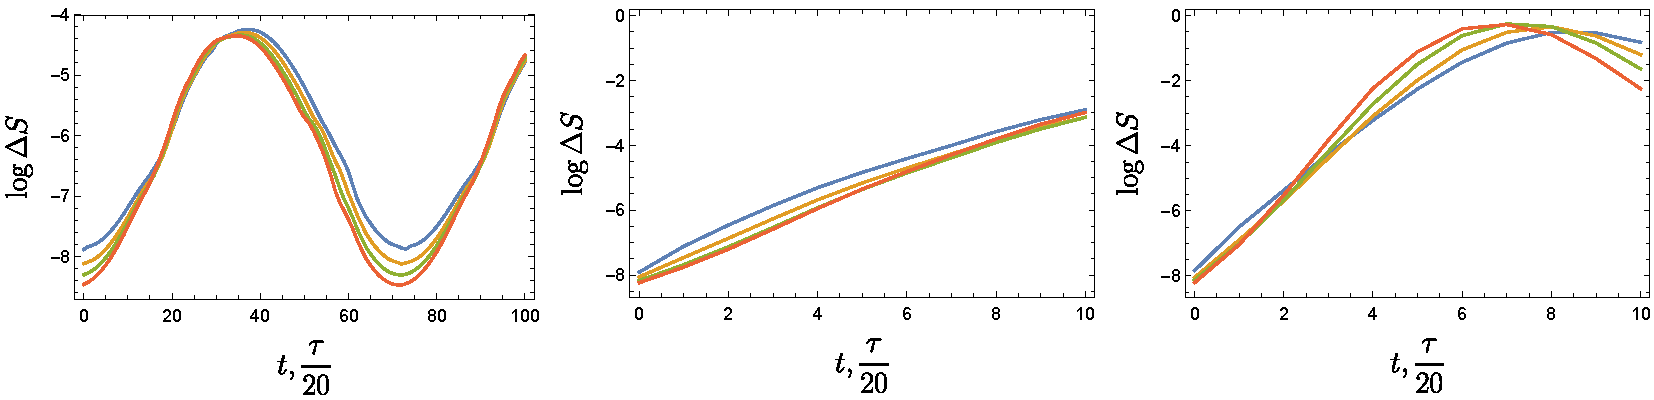
\includegraphics[width=1.0\textwidth]{figures/lyapunovs.pdf}
  \end{figure}
  
  \begin{center}
      \begin{tabular}{c|c|c|c}
        $\tau$ & $2 \ T_r$ & $7.5 \ T_r$ & $12 \ T_r$ \\ \hline
        $\lambda$ & $0.0$ & $1.62 \ f_r$ & $1.84 \ f_r$
      \end{tabular}
  \end{center}
    
  \phantom{42}
  
  \textbf{Chaos is possible!}. \\
  Thus, length of fiber from numerical analysis. $L \sim 1 \ \text{m}$
  
\end{frame}

\section{Branches of Light}
\frame{
\frametitle{The other idea in nature}

\begin{figure}[h]
    \centering
    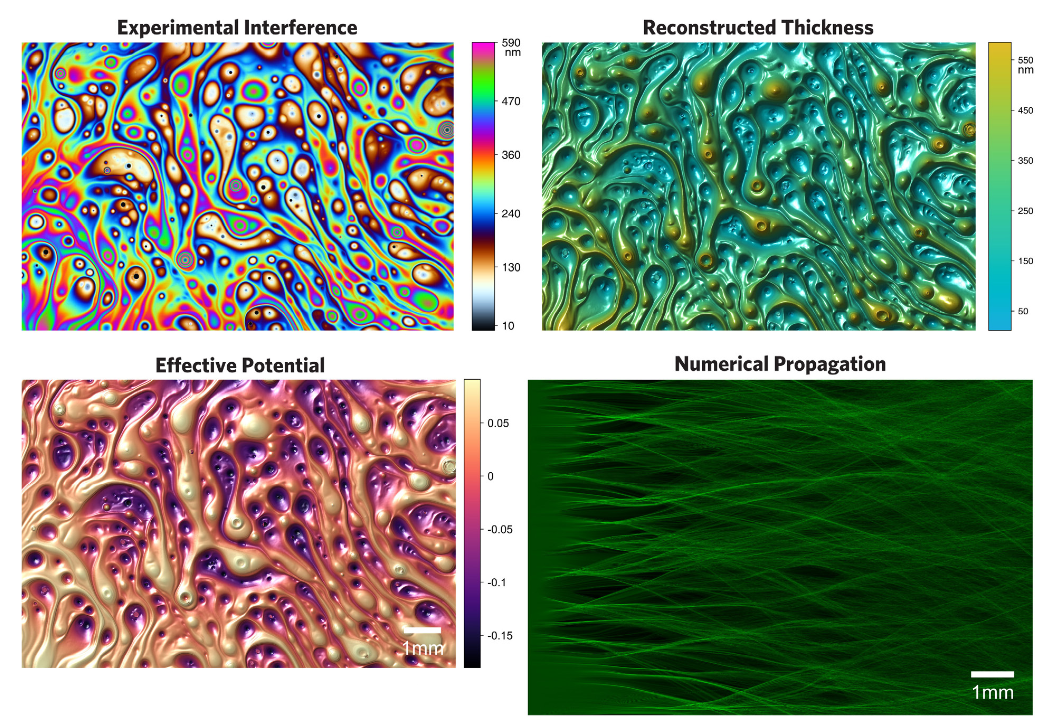
\includegraphics[width=0.8\textwidth]{images/nature_article.png}
    %\label{fig:}
\end{figure}
\textit{Patsyk, A., Sivan, U., Segev, M. et al. "Observation of branched flow of light". Nature 583, 60–65 (2020).}}

\frame{
\frametitle{Theory of refraction index}
\begin{minipage}{0.35\textwidth}
    \begin{figure}[h]
    \centering
    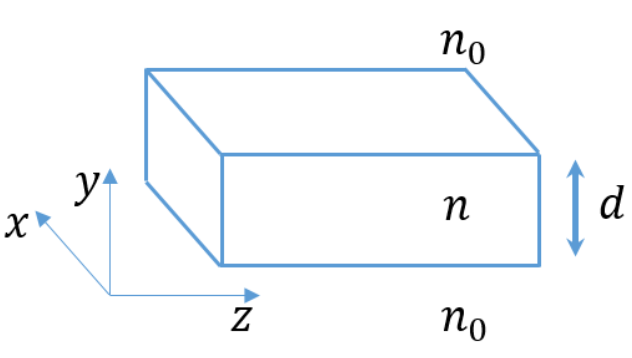
\includegraphics[width=1\textwidth]{images/nature_scheme.png}
    %\label{fig:}
\end{figure}
\end{minipage}
\hfill
\begin{minipage}{0.55\textwidth}
	The Helmholtz equation again
	\begin{equation*}
		\Delta E + k_0^2 n^2(y) E = 0
	\end{equation*}    
	while solving like $E = \psi(x,z) G(y)$ gives a solutions:
\end{minipage}
	\begin{equation*}
		\partial_{y y}G + k_0^2 n^2(y) G = k_0^2 n^2_{\text{eff}} G,
	\hspace{1 cm}
		\nabla_{\perp}^2 \psi + k_0^2 n_\text{eff}^2 \psi = 0.
	\end{equation*}
	And solving the left one we obtain
	\begin{equation*}
		k_0^2 y \sqrt{n_\text{soap}^2 - n_\text{eff}^2} + 2 \arctan\left(\frac{\sqrt{n_\text{soap}^2 - n_\text{eff}^2}}{\sqrt{n_\text{eff}^2 - n_\text{air}^2}}\right) - \pi(m+1) = 0.
	\end{equation*}
}

% 

\frame{
The beam goes to the film through the optical fiber:

\phantom{42}

\begin{minipage}{0.45\textwidth}
    \begin{center}
        \incfig{scheme8}    
    \end{center}
\end{minipage}
\hfill
\begin{minipage}{0.45\textwidth}
    \begin{figure}[h]
        \centering
        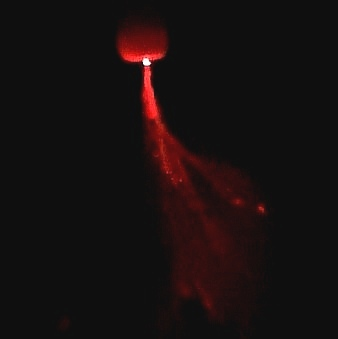
\includegraphics[width=0.99\textwidth]{figures/photo3.jpg}
        %\caption{}
        %\label{fig:}
    \end{figure}
\end{minipage}

\phantom{42}

Light scattering occurs most likely on micro bubbles and other inhomogeneities inside the solution. \frametitle{Experimental setup}}

\frame{


After outlet of the optical fiber ($d_{\text{core}} \sim 50 \, \mu$m) light really starts branching.

\begin{figure}[h]
    \animategraphics[loop, controls=play,width=0.52\textwidth]{20}{gifs/g2/}{1}{100} 
    \hspace{5 mm} 
    \animategraphics[loop, controls=play,width=0.3\textwidth]{20}{gifs/g1/}{1}{54} 
\end{figure}

The effect of the thickness of the film on the system dynamics is noticeable. After the time expires, the film becomes thinner, the rays are actively branched. \frametitle{Film dynamics}}

\frame{
To demonstrate branching, consider the movement of light in the environment with 
$n(x, y) = \textstyle\frac{1}{3}\left(\cos x +\cos y \right) + 2$.

% \phantom{42}

\begin{minipage}{0.6\textwidth}
      \begin{figure}[h]
      \animategraphics[loop,controls=play,width=0.99\textwidth]{20}{gifs/g3/}{1}{63}
    \end{figure}
\end{minipage}
\hfill
\begin{minipage}{0.35\textwidth}
    \begin{figure}[h]
        \centering
        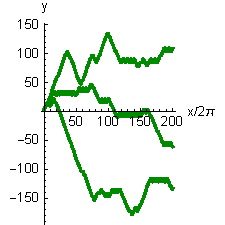
\includegraphics[width=1.0\textwidth]{figures/rnd_walk.pdf}
        %\caption{}
        %\label{fig:}
    \end{figure}

     \phantom{42}
\end{minipage}

This happens random walk across heterogeneous media. \frametitle{Modeling}}

\frame{
Walk in periodic media can be reduced to the billiard table.

\begin{minipage}{0.5\textwidth}
      \begin{figure}[h]
      \animategraphics[loop,controls=play,width=0.99\textwidth]{20}{gifs/g4/}{1}{200} 
    \end{figure}
\end{minipage}
\hfill
\begin{minipage}{0.45\textwidth}
For almost all trajectories:
    \begin{itemize}
        \item[\textcolor{mygreen}{\checkmark}] ergodic behaviour;
        \item[\textcolor{mygreen}{\checkmark}] positive Lyapunov exponent;
        % \item[\textcolor{mygreen}{\checkmark}] .
    \end{itemize}
    so we have pretty example of dynamical chaotic system.
\end{minipage}


That can be considered as a smoothed version of Lorentz gas or Sinai billiard. \frametitle{Sinai billiard}}


% % \section{Slow adder}






\section{Results}

\frame{

\begin{minipage}{0.75\textwidth}
      We tried to use partially finished decision for video transmission:
    \begin{center}
        \incfig{scheme7}    
    \end{center}
\end{minipage}
\hfill
\begin{minipage}{0.2\textwidth}
    \begin{tabular}{c|c}
     $\tau_\text{i} / \tau_{\text{r}}$ & $\lambda \tau_{\text{r}}$ \\
     \hline
     0 & 1.62 \\ 
     2 & 0.71 \\
     6 & 0.11 \\
     10 & $\to \const$ \\
     % 10& 0.00 \\
    \end{tabular}

    \phantom{42}

    \textit{Observed} the constant \\ behavior.
\end{minipage}


% In theory, it is enough to turn around (or navigate through the amplifier) several clems, 
% what is planned to be implemented after more thorough preparation.

% \vspace{2mm}
The system is designed for oscillations $< 20$ MGz, so
\vspace{-2mm}
\begin{equation*}
    \hspace{-5mm}
    S(t - \tau) \to \int_{0}^{\tau_\text{i}} f(\eta) S(t-\eta) \d\eta,
    \hspace{2.5 mm} 
    \tau_\text{i} \approx 50 \tau_{\text{r}} > 5 \tau_{\text{r}},
    \hspace{0.1cm} \Rightarrow \hspace{0.1cm}
    \lim_{t \to \infty} S(t-\tau) = \const
\end{equation*}

% написать про МГц -- интегрирование по n tau.

% 10 Мгц 
% 10-20 tau

% 
% tau_i -> 
% 200 Мгц -- максимум, 

% или слайд, или там же ---
% про Lyap(tau_i) зависимость
% \frametitle{Alternative implementations}}


\frame{
As a result of the project:
\begin{itemize}
    \iitem{According to the equations of the laser's evolution with a feedback, the \textbf{numerical model was built} in the ideal and non ideal case.}
    \iitem{It is shown that \textbf{chaos is possible in the system}. Chaos parameters are estimated. The frequency limitation were evaluated for the system. }
    \iitem{A scheme of positive feedback has been developed and built. The optimal parameters for the scheme were selected.}
    \iitem{Got prepared for the use of an industrial setup.}
\end{itemize}

 \frametitle{Problems}}

\appendix
\section{Additional Material}

\frame[noframenumbering]{
To start the laser idea we need to obtain:
\begin{itemize}
	\iitem{Solution of the Schr\"odinger equation in a semiconductor medium for the wavefunction of an electron;}
	\iitem{Induced polarization for distribution of holes and electrons in a semiconductor;}
	\iitem{Interaction of electrons in a semiconductor with an wave equation and outer electric field.}
\end{itemize}
 \frametitle{The concept of a semiconductor laser}}

\frame[noframenumbering]{
We will need the Schr\"odinger equation:
\begin{equation*}
	H_{\text{crystal}} \Psi_n(\vc{r}) = \left[\frac{\vc{p}^2}{2 m_0} + U_p(\vc{r})\right] \Psi_n(\vc{r})
\end{equation*}
where $\vc{p} = - i \hbar \nabla$ is the momentum operator, $m_0$ is the free electron mass, $U_p(\vc{r})$ is th periodic potential of the bulk semiconductor.

The solution is the Bloch function:
\begin{equation*}
	\Psi_{n, \smallvc{k}}(\vc{r}) = u_{n, \smallvc{k}}(\vc{r}) \frac{1}{\sqrt{V}} e^{i \smallvc{k} \cdot \smallvc{r}}.
\end{equation*}
 \frametitle{Electronic states in a semiconductor}}

\frame[noframenumbering]{
In case of an optical field the Hamiltonian changes to
\begin{equation*}
	H = \frac{[\vc{p} + e \vc{A}(\vc{r}, t)]^2}{2 m_0} + U_p(\vc{r}) = H_\text{crystal} + H'
\end{equation*}
$\vc{A}(\vc{r},t)$ is the vector potential of the optical field. So the interaction Hamiltonian 
\begin{equation*}
	H' \approx \frac{e}{m_0} \vc{A}(\vc{r},t) \cdot \vc{p}.
\end{equation*} \frametitle{Hamilton in an outer field}}

\frame[noframenumbering]{
For y-propagating field: $E(\vc{r}, t) = \frac{1}{2} E_0 e^{i (\beta y - \omega t)} + \const$ the Hamiltonian is
\begin{equation*}
	H' = \frac{1}{2} \mu(k_q,x,z) [E_0 e^{i (\beta y - \omega t)} + \const]
\end{equation*}
where $\mu$ is the transition matrix that describes the semiconductor, $k_q$ -- quantized wavevector of the electron. \frametitle{Hamilton in an outer field}}

\frame[noframenumbering]{
As one can obtain after rewritten density matrix in terms of carrier distributions, and in order avoid irrelevantly enormous formulas we get polarization as:
\begin{equation*}
	\mathcal{P}_{in}(\vc{r}, t) = \frac{1}{2} \mathcal{P}_{in,0} e^{i (\beta y - \omega t)} + \const =
\end{equation*}
\begin{equation*}
	= - \sum \frac{\xi(\vc{r},k_q, x, z)}{V(k_q, x, z)}[\rho_{eh}(k_q, x, z)\mu(k_q, x, z) + \const]	
\end{equation*}
where $V(k_q, x, z)$ is the confinement volume of electrons and holes and
\begin{equation*}
	\xi(\vc{r}, k_q, x, z) = 
	\left\{ \begin{aligned}
		&1, \ \vc{r} \text{ inside V}\\
		&0, \ \vc{r} \text{ outside V}
	\end{aligned}
	\right.
\end{equation*}

 \frametitle{Induced polarization in an outer field}}

\frame[noframenumbering]{
For the wave porpagating along the y direction in active layer the equation is:
\begin{equation}
	\triangle E(\vc{r},t) - \mu_0 \varepsilon(\vc{r}) \frac{\partial^2}{\partial t^2} E(\vc{r}, t) = \mu_0 \frac{\partial^2}{\partial t^2} P_{in}(\vc{r},t)
	\label{1.46}
\end{equation}
The partial solution for this equation we will be searching in a form of
\begin{equation*}
	E(\vc{r}, t) = A_0(t) E_{\text{eig}}(x,z) = \frac{1}{2} E_0 e^{i (\beta y - \omega t)} + \const.
\end{equation*} \frametitle{Injection the light}}

\frame[noframenumbering]{
Substituting in wave equation\eqref{1.46} the obtained polarization and solution for $E(\vc{r}, t)$ and assuming that $A(t)$ changes slowly we get
\begin{equation}
	\frac{d A_0}{d t} = \frac{i \omega}{2 \varepsilon_0 n_r^2} A_0 \sum_{k_q, x, z}\Gamma_{MD} \frac{1}{V_{MD}} |\mu(k_q, x, z)|^2[\rho_{ee} + \rho_{hh} - 1]
\end{equation}
where 
\begin{equation*}
	\Gamma_{MD} = \frac{\varepsilon(x,z) |E_0(x,z)|^2}{\iint \varepsilon(x,z) |E_0(x,z)|^2 dx d z}\bigg|_{x,z=0,0}
\end{equation*}
is a \textit{dimensional coupling factor}. \frametitle{Partial solution part}}

\frame[noframenumbering]{
Now we can rewrite
\begin{equation}
	\frac{d A_0}{d t} = \frac{1}{2} v_g [\Gamma_{MD}G - i \Gamma_{MD} N_r]A_0,
\end{equation}
where $v_g = c/n_r$ for $c$ -- the speed of light in vacuum, and $n_{r}$ -- refraction coefficient. We will call the \textit{gain coefficient} $g = \Gamma_{MD}G$.
From Schr\"odinger equation we obtain the photon density as:
\begin{equation*}
	S = \frac{1}{2} \frac{\varepsilon_0 n_r^2 |A_0 E(0)|^2}{E_0}.
\end{equation*} \frametitle{Getting the solution}}

\frame[noframenumbering]{
Using the equation for $A_0$ we obtain for the photon density (real part):
\begin{equation}
	\frac{d S}{d t} = v_g \Gamma_{MD} G(E) S.
\end{equation}

Total optical power in the active region:
\begin{equation*}
	-\int E(\vc{r},t) \frac{d \mathcal{P}_{in}(\vc{r},t)}{d t} d \vc{r} = - \hbar \omega V_{MD} \frac{d N_{MD}}{d t},
\end{equation*}
which leads to electrons (holes) density (complex part):
\begin{equation}
	\frac{d N_{MD}}{d t} = - v_g G(E) S.
\end{equation} \frametitle{The laser equations}}

\frame[noframenumbering]{
Irrelevantly enormous
formulas if someone really need it:

\begin{equation*}
	\frac{d}{d t}[\rho_{ee}(k_q, x, z)] = \frac{i}{\hbar}[H' \rho_{eh}(k_q, x, z) - \const] - \frac{\rho_{ee}(k_q, x, z) - f_e}{\tau_e},
\end{equation*}
\begin{equation*}
	\frac{d}{d t}[\rho_{hh}(k_q, x, z)] = \frac{i}{\hbar}[H' \rho_{eh}(k_q, x, z) - \const] - \frac{\rho_{hh}(k_q, x, z) - f_e}{\tau_e},
\end{equation*}
\begin{equation*}
	\frac{d}{d t}[\rho_{eh}(k_q, x, z)] = \frac{i}{\hbar} H'[\rho_{ee} + \rho_{hh} - 1] - \frac{i}{\hbar} E_{tr} \rho_{e h} - \frac{\rho_{eh}}{T_{deph}}.
\end{equation*} \frametitle{Carrier density in an outer field}}

\frame[noframenumbering]{
And from the previous equation we can describe the quantum well laser behavior
\begin{equation*}
	\frac{d S}{d t} = \Gamma(0) G_0 v_g S - \frac{S}{\tau_p}. 
\end{equation*}
\begin{equation*}
	\frac{d N}{d t} = \frac{J}{e} - \frac{N}{\tau_n} - \Gamma G_0 v_g S.
\end{equation*} \frametitle{The laser equations}}

\frame[noframenumbering]{
\textbf{Thr.} If there is no stationary points on the enclosed 2D region $G$ and some trajectory exists $\gamma \subset G$, then $\gamma$ is a closed loop path or tends to the closed one.

But there is still a hope for a chaos!

We add positive optoelectronic feedback in order to raise to 3D our equation.
\begin{align*}
	&\frac{d S}{d t} = v_g g S - \gamma_p S,\\
	&\frac{d N}{d t} = \frac{J}{e}[1 + \frac{\xi S(t-\tau)}{S_0}] - \gamma_n N - g S.
\end{align*} \frametitle{Poincar\'e-Bendixson theorem}}

\frame[noframenumbering]{
\begin{minipage}{0.45\textwidth}
    
\end{minipage}
\hfill
\begin{minipage}{0.45\textwidth}
    \begin{center}
        \incfig{scheme2}
    \end{center}
\end{minipage}

 \frametitle{Range}}


\end{document}



